\documentclass{beamer}

\usetheme{Darmstadt}
\usepackage{amsfonts}
\usepackage{graphics,xcolor}
\usepackage{stmaryrd,amssymb,amsmath}
\usepackage[most]{tcolorbox}
\newtcolorbox{lol}[1]{colback=red!5!white,colframe=red!75!black,fonttitle=\bfseries,title=#1,breakable}
\usepackage{docmute}
\usepackage{hyperref}
\usepackage{graphicx}
%\usepackage{unicode-math}
\newcommand{\nat}{\mathbb{N}}
\newcommand{\ints}{\mathbb{Z}}
\newcommand{\intersection}{\ensuremath{\cap}}
\newcommand{\emptyword}{\ensuremath{\epsilon}}
\newcommand{\len}[1]{\ensuremath{|#1|}}
\newcommand{\union}{\ensuremath{\cup}}
\newcommand{\deltahat}{\ensuremath{\widehat{\delta}}}


\title{Queries in the model}

\author{Balaji}
\date{}
\institute{IISc Bangalore}
\begin{document}
\maketitle
\begin{frame}{What I have implemented so far}
    \begin{itemize}
        \item Wrote code to generate the smile nature of implied volatility of calls and puts of 5 weeks of NIFTY 50 index options.
        \item Generated the implied volatility surface using linear interpolation.
        \item Wrote code to calculate the call price function using the Black-Scholes formula.
        \item From this I generate the volatility surface using Dupire's formula.
        \item Then I usee the model to estimate the stock at given timesteps.
    \end{itemize}
\end{frame}
\begin{frame}{What I have implemented so far}
    \begin{center}
    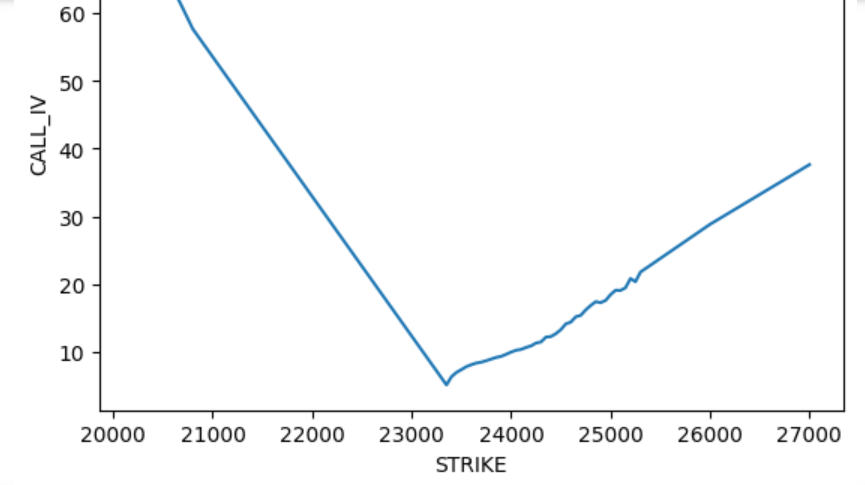
\includegraphics[scale = 0.25]{IV_call}
    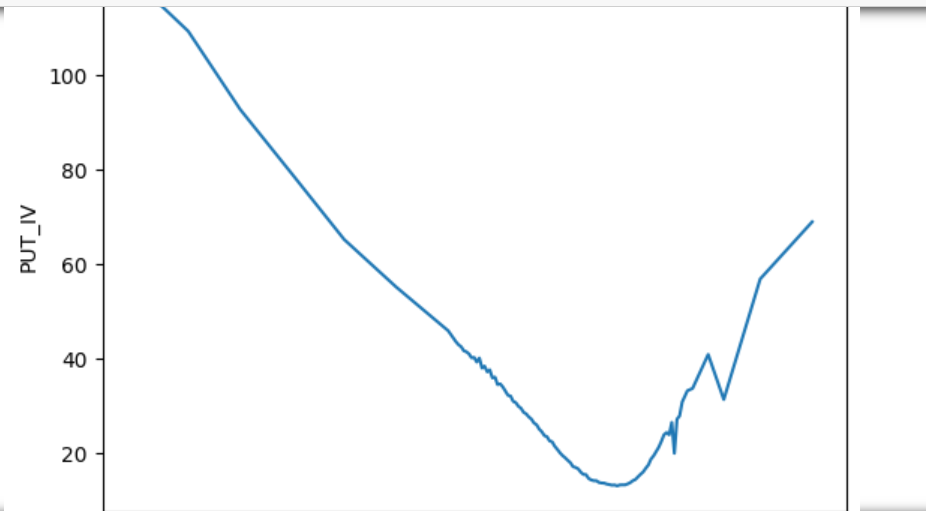
\includegraphics[scale = 0.25]{IV_put}
    \end{center}
\end{frame}
\begin{frame}{What I have implemented so far}
    \begin{center}
    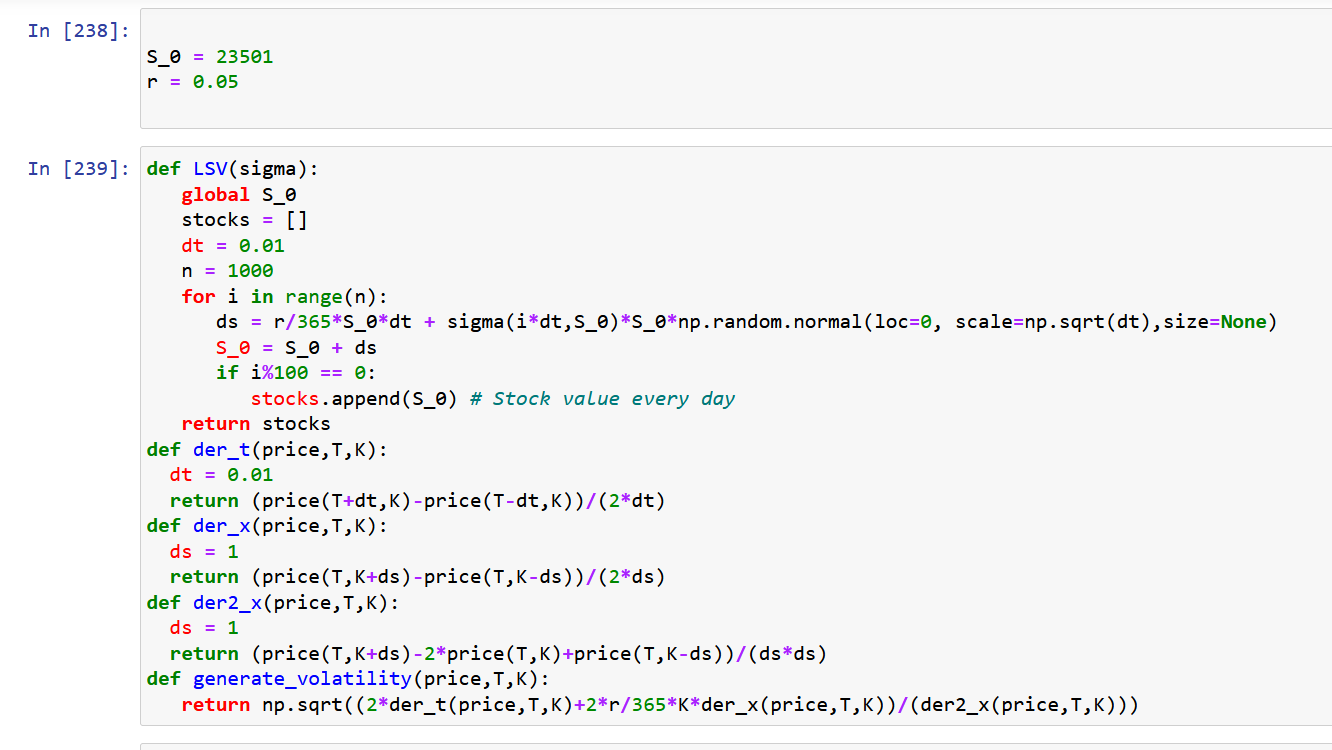
\includegraphics[scale = 0.25]{model_surface}
    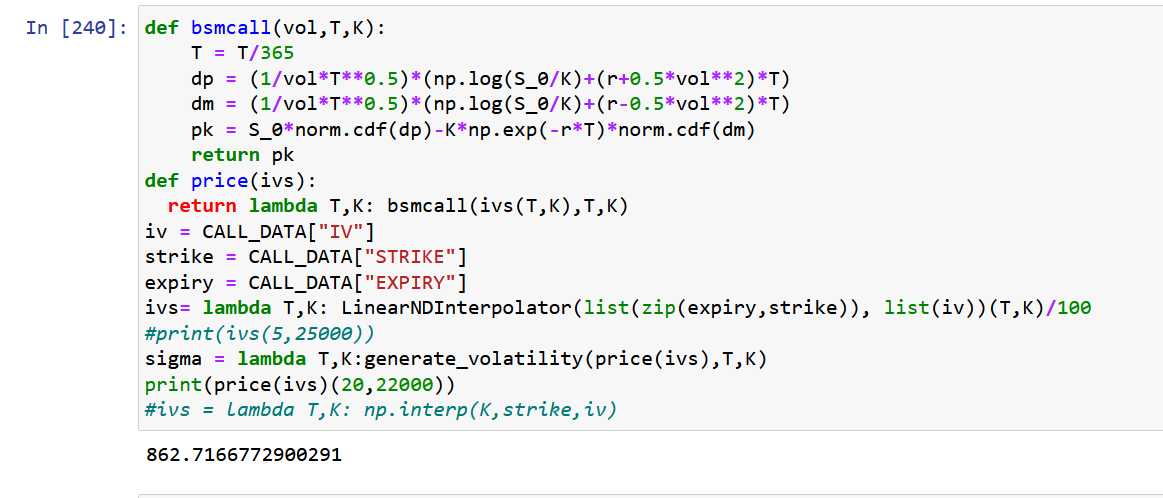
\includegraphics[scale = 0.25]{IVS}
    \end{center}
\end{frame}
\begin{frame}{What is working and what is not}
\begin{itemize}
    \item Successfully generated the smile for 5 weeks of call and put options.
    \item Successfully generated the implied volatility surface using linear interpolation.
    \item Price obtained from the Black-Scholes formula is not matching with the actual price and is even giving negative prices for high strikes of call options.
\end{itemize}
\end{frame}
\end{document}